\chapter{Thiết Kế và Lắp Đặt Hệ Thống}
\label{ch:hardware_architecture}

\section{Tổng Quan Kiến Trúc Hệ Thống}
Hệ thống FloodGuard gồm 5 khối chức năng chính được tích hợp đồng bộ:
\begin{enumerate}
    \item \textbf{Khối xử lý trung tâm:} Vi điều khiển ESP32 DevKit V1 với chip lõi kép Xtensa 32-bit (tần số xung nhịp $240\,\text{MHz}$), tích hợp bộ nhớ SRAM $520\,\text{KB}$ và kết nối không dây Wi-Fi $802.11\,\text{b/g/n}$, đảm nhiệm đồng thời tác vụ đo đạc thời gian thực, thuật toán FSM và máy chủ Web Server nhúng.
    \item \textbf{Khối cảm biến (Sensors):} Cảm biến siêu âm HC-SR04 đo khoảng cách tới mặt nước hồ thu và cảm biến mưa FC-37 (tấm điện cực kết hợp mạch so sánh LM393) đo lượng nước mưa bề mặt.
    \item \textbf{Khối chấp hành (Actuators):} Gồm hai cơ cấu chấp hành độc lập: Động cơ Servo SG90 điều khiển góc mở cửa van xả lũ ($0^\circ - 90^\circ - 180^\circ$) và Module Relay $5\,\text{V}$ điều khiển đóng/ngắt máy bơm mini thoát nước.
    \item \textbf{Khối cảnh báo tại chỗ (Signaling):} Cụm 3 đèn LED màu (Xanh, Vàng, Đỏ) và còi báo động Active Buzzer $5\,\text{V}$.
    \item \textbf{Khối máy tính vận hành (Operator PC/Laptop):} Trạm máy tính kết nối không dây qua sóng Wi-Fi SoftAP để mở giao diện Web Dashboard giám sát và can thiệp điều khiển; đồng thời kết nối có dây qua cổng Micro-USB phục vụ nạp firmware PlatformIO và theo dõi Serial Debug Monitor.
\end{enumerate}

\section{Giải Pháp Điều Khiển Qua Mạng Không Dây Cục Bộ Thay Cho Nút Nhấn Cơ Học}

Trong thiết kế trạm FloodGuard, giao diện giám sát và điều khiển can thiệp được chuyển dịch hoàn toàn sang \textbf{giao diện Web Dashboard thông qua mạng không dây cục bộ (Local Wi-Fi / SoftAP)} thay cho các nút bấm vật lý tại chỗ. Giải pháp này xuất phát từ các lập luận kỹ thuật và thực tiễn vận hành:
\begin{itemize}
    \item \textbf{Đảm bảo an toàn tính mạng cho người vận hành:} Mục tiêu cốt lõi của trạm bơm chống ngập là vận hành tự trị $24/7$. Khi xảy ra thiên tai mưa bão ngập lụt, khu vực hồ thu và trạm bơm tiềm ẩn nguy cơ giông sét đánh, sụt lở mép bờ và rò rỉ điện từ các đường dây động lực ngâm trong nước. Việc điều khiển không dây cho phép kỹ thuật viên đứng từ vị trí khô ráo an toàn (trong xe chỉ huy hoặc trên tầng cao tòa nhà cách trạm $15 - 30\,\text{m}$) để theo dõi và ra lệnh.
    \item \textbf{Cung cấp đầy đủ ngữ cảnh dữ liệu trước khi can thiệp:} Khác với nút bấm vật lý vốn chỉ cho phép thao tác "mù" mà không biết chính xác mực nước hay trạng thái van xả, Web Dashboard hiển thị toàn bộ đồ họa số hóa (phần trăm nước, khoảng cách cm, cấp độ mưa, trạng thái FSM). Người vận hành có đầy đủ cơ sở thông tin kỹ thuật trước khi quyết định kích hoạt máy bơm hoặc xoay van xả lũ.
    \item \textbf{Phân tích rủi ro \& Giải pháp Dừng khẩn cấp (Emergency Stop):}
    Việc không trang bị nút bấm cơ học đồng nghĩa với việc nếu thiết bị di động hết pin hoặc mạng Wi-Fi bị nhiễu sóng nặng, người tại chỗ không thể can thiệp tức thời. Để giảm thiểu rủi ro này:
    \begin{itemize}
        \item Trong mô hình thực nghiệm, hệ thống áp dụng cơ chế bảo vệ Failsafe tự động chuyển về \texttt{AUTO} sau $30\,\text{s}$ mất kết nối và tự động kích hoạt bơm toàn tải nếu nước chạm mức nguy cấp CRITICAL.
        \item Tuy nhiên, theo các tiêu chuẩn an toàn máy móc công nghiệp (ISO 13850 và IEC 60204-1), ở phiên bản sản xuất thương mại thực tế ngoài hiện trường, hệ thống khuyến nghị bắt buộc bố trí thêm \textbf{01 nút Dừng khẩn cấp cơ học (E-Stop Button)} dạng nấm màu đỏ có chốt khóa, đấu ngắt trực tiếp nguồn điện cấp cho cuộn hút Relay của máy bơm nhằm xử lý sự cố kẹt rác cơ học hoặc cháy nổ động cơ tại chỗ.
    \end{itemize}
\end{itemize}

\section{Bảng Phân Công Chân GPIO}
\begin{table}[H]
\centering
\caption{Bảng phân công chân phần cứng trên vi điều khiển ESP32}
\label{tab:gpio_mapping}
\begin{tabularx}{\textwidth}{c l l l X}
\toprule
\textbf{STT} & \textbf{Thiết bị / Module} & \textbf{Chân tín hiệu} & \textbf{GPIO ESP32} & \textbf{Chức năng kỹ thuật \& Lưu ý điện áp} \\
\midrule
1 & HC-SR04 (Siêu âm) & Trig & \texttt{GPIO 13} & Phát xung kích siêu âm $10\,\mu\text{s}$ ($3.3\,\text{V}$) \\
1 & HC-SR04 (Siêu âm) & Echo & \texttt{GPIO 12} & Nhận xung phản hồi (Strapping Pin MTDI; hạ áp $5\,\text{V} \to 3.3\,\text{V}$) \\
2 & Cảm biến mưa FC-37 & DO (Digital) & \texttt{GPIO 34} & Ngõ vào số báo mưa/khô (Input-only, không pull-up nội) \\
2 & Cảm biến mưa FC-37 & AO (Analog) & \texttt{GPIO 35} & Đo điện áp tương tự qua ADC1\_CH7 (Input-only) \\
3 & Động cơ Servo SG90 & PWM & \texttt{GPIO 27} & Xung PWM điều khiển van xả ($0^\circ - 90^\circ - 180^\circ$) \\
4 & Module Relay 5V & IN & \texttt{GPIO 23} & Kích đóng/ngắt máy bơm 5V -- \textbf{Active LOW} \\
5 & LED Đỏ (Nguy cấp) & Anode (+) & \texttt{GPIO 18} & Báo động CRITICAL / DANGER (nối tiếp $R = 220\,\Omega$) \\
6 & LED Vàng (Cảnh báo) & Anode (+) & \texttt{GPIO 19} & Báo trạng thái WARNING (nối tiếp $R = 220\,\Omega$) \\
7 & LED Xanh (An toàn) & Anode (+) & \texttt{GPIO 21} & Báo trạng thái NORMAL (nối tiếp $R = 220\,\Omega$) \\
8 & Còi Active Buzzer 5V & Cực (+) & \texttt{GPIO 4} & Phát xung âm thanh cảnh báo đa cấp độ \\
\bottomrule
\end{tabularx}
\end{table}

\section{Sơ Đồ Nguyên Lý Mạch Điện \& Kết Nối Ngoại Vi}

Sơ đồ nguyên lý mạch điện chi tiết kết nối giữa vi điều khiển ESP32 với toàn bộ cảm biến, cơ cấu chấp hành, thiết bị chỉ thị và máy tính vận hành được minh họa trong Hình~\ref{fig:circuit_diagram}.

\begin{figure}[H]
    \centering
    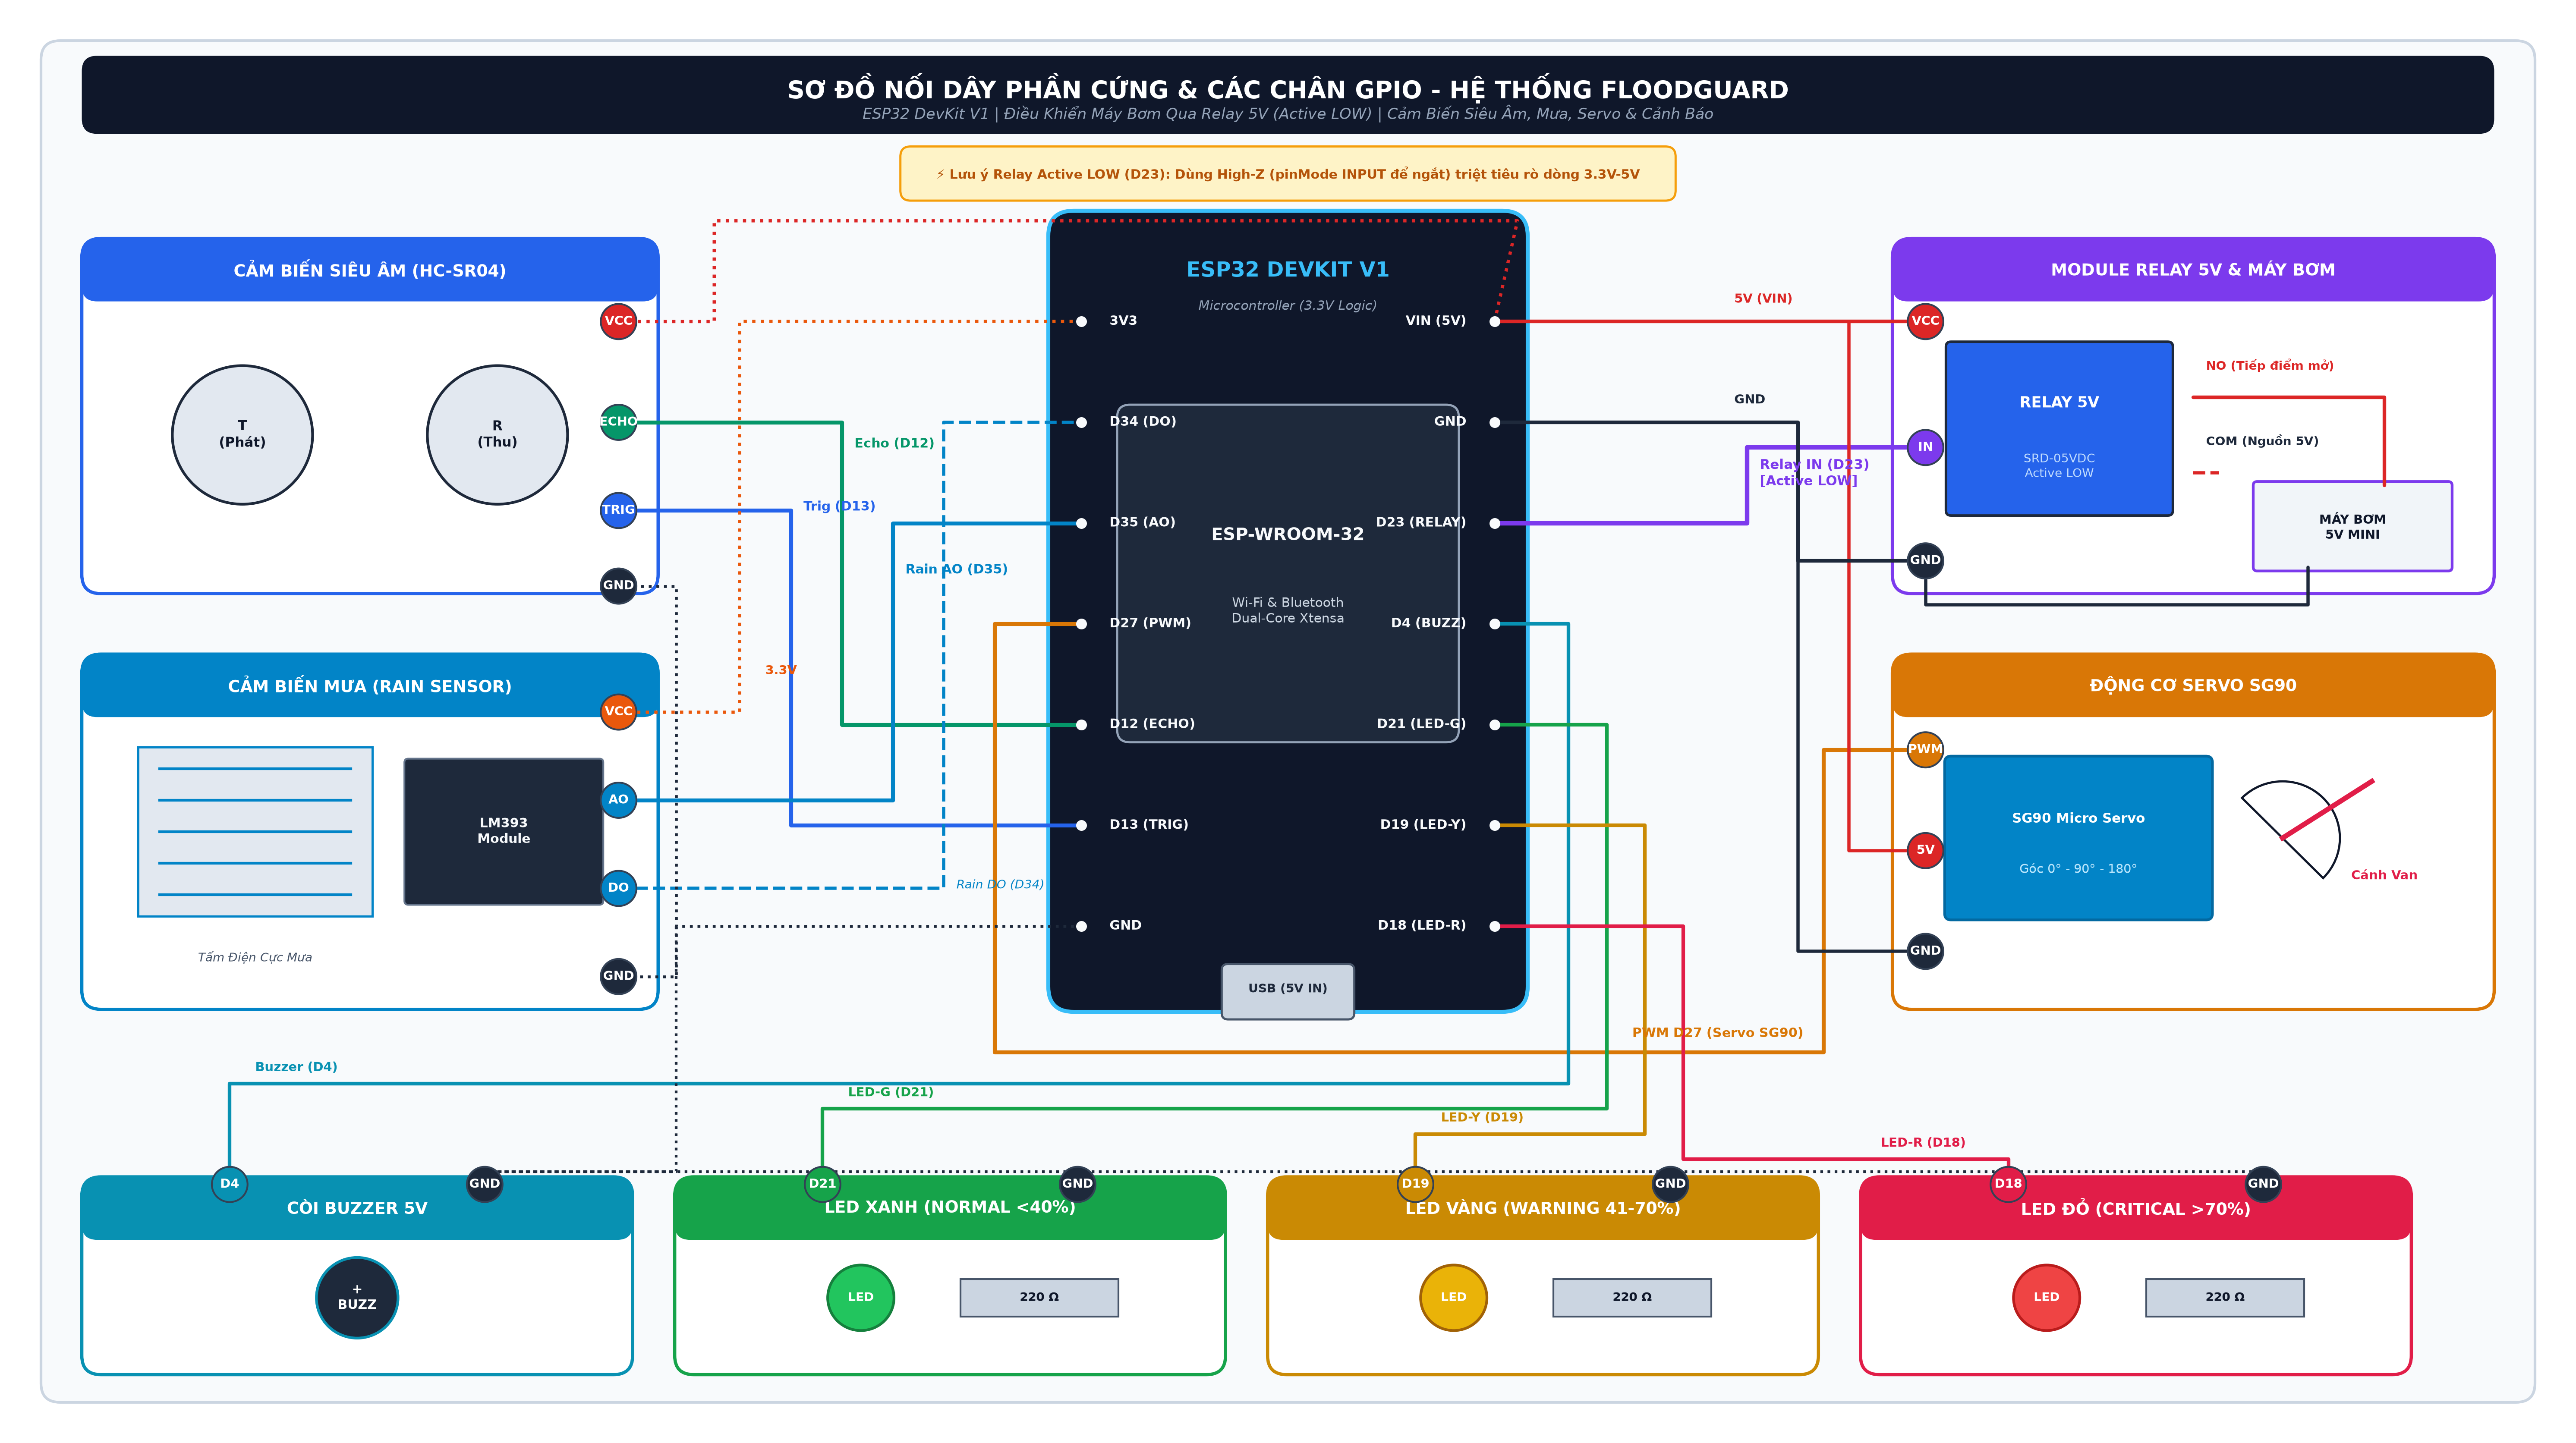
\includegraphics[width=\textwidth]{figures/circuit_diagram.png}
    \caption{Sơ đồ nguyên lý mạch điện chuẩn IEC và phân vùng các khối chấp hành trạm FloodGuard}
    \label{fig:circuit_diagram}
\end{figure}

Dựa trên sơ đồ nguyên lý nối dây và phân vùng các khối chấp hành, các nguyên lý phối ghép phần cứng và giải pháp bảo vệ mạch điện được phân tích chi tiết:

\subsection{Khối Chấp Hành Công Suất: Relay 5V, Diode Flyback \& Nguồn Cấp Máy Bơm}
Máy bơm nước mini $5\,\text{V}$ sử dụng động cơ DC có chổi than, tiêu thụ dòng điện làm việc định mức khoảng $0.5 - 0.8\,\text{A}$ và có thể lên tới $1.5\,\text{A}$ khi khởi động (\textit{Inrush current}). Để vận hành an toàn:
\begin{itemize}
    \item \textbf{Phân tách nguồn cấp động lực:} Nguồn cấp cho máy bơm được lấy từ chân \texttt{VIN} (nối với bộ nguồn $5\,\text{V} - 2\,\text{A}$ bên ngoài), tuyệt đối không lấy từ chân \texttt{3V3} của ESP32 nhằm tránh hiện tượng sụt áp gây khởi động lại vi điều khiển (\textit{Brown-out Reset}).
    \item \textbf{Bảo vệ cách ly quang (Optocoupler) \& Diode dập xung ngược (Flyback Diode):} Module Relay tích hợp optocoupler PC817 cách ly hoàn toàn điện áp $3.3\,\text{V}$ của vi điều khiển với cuộn hút $5\,\text{V}$. Cuộn hút Relay được mắc song song với một Diode dập xung ngược (\textit{Flyback Diode}) phân cực ngược để triệt tiêu sức điện động cảm ứng $e = -L\frac{di}{dt}$ sinh ra khi ngắt dòng điện cuộn dây, ngăn chặn xung điện áp cao đánh thủng transistor kích mở.
    \item \textbf{Cơ chế điều khiển Active LOW kết hợp trạng thái High-Z:}
    Module Relay đóng tiếp điểm khi chân tín hiệu \texttt{IN} được kéo xuống mức \texttt{LOW} ($0\,\text{V}$). Do vi điều khiển ESP32 chỉ xuất mức \texttt{HIGH} ở $3.3\,\text{V}$, sự chênh lệch $5\,\text{V} - 3.3\,\text{V} = 1.7\,\text{V}$ có thể làm rò dòng qua LED phát quang nội của optocoupler khiến Relay không nhả hoàn toàn. Hệ thống xử lý triệt để hiện tượng này bằng cách:
    \begin{itemize}
        \item Khi bật bơm: Cấu hình ngõ ra \texttt{OUTPUT} và kéo chân Relay xuống mức \texttt{LOW} ($0\,\text{V}$).
        \item Khi ngắt bơm: Cấu hình ngõ vào \texttt{INPUT} thả nổi chân về trạng thái trở kháng cao (High-Z).
    \end{itemize}
\end{itemize}

\subsection{Khối Cảm Biến: Bảo Vệ Điện Áp Echo \& Chân Strapping GPIO 12}
\begin{itemize}
    \item \textbf{Cảm biến siêu âm HC-SR04 (GPIO 13 Trig, GPIO 12 Echo):}
    Cảm biến HC-SR04 sử dụng nguồn cấp $5\,\text{V}$. Chân \texttt{Echo} xuất ra xung vuông mức biên độ $5\,\text{V}$. Do các chân GPIO của ESP32 chỉ dung nạp điện áp tối đa $3.3\,\text{V}$, chân \texttt{Echo} được mắc qua mạch phân áp trở hoặc điện trở hạn dòng bảo vệ kết hợp diode kẹp áp nội của vi điều khiển để hạ mức điện áp an toàn xuống $\approx 3.3\,\text{V}$. Về mặt vật lý lắp đặt, cảm biến có vùng mù ở khoảng cách $< 3\,\text{cm}$ và góc phát chùm tia hình nón $\pm 15^\circ$; do đó khi gá đặt trên mô hình thực nghiệm, mặt loa cần đặt cao hơn mức nước đầy tối đa ít nhất $5 - 6\,\text{cm}$ và chiếu thẳng vào tâm bể để tránh dội sóng nhiễu vào thành bể.
    \item \textbf{Lưu ý kỹ thuật đặc biệt với chân Strapping MTDI (GPIO 12):}
    Trên vi điều khiển ESP32, \texttt{GPIO 12} là chân cấu hình khởi động (\textit{Strapping Pin MTDI}). Tại thời điểm cấp nguồn/reset, chip sẽ đọc mức logic của chân này: nếu ở mức \texttt{LOW}, chip chọn điện áp cấp cho bộ nhớ SPI Flash nội là $3.3\,\text{V}$ (bình thường); nếu bị kéo lên mức \texttt{HIGH}, chip chuyển sang chế độ Flash $1.8\,\text{V}$ dẫn tới treo vi điều khiển (vòng lặp Boot loop). Trong mạch thiết kế, chân \texttt{Echo} của cảm biến HC-SR04 ở trạng thái nghỉ luôn duy trì mức \texttt{LOW} ($0\,\text{V}$), do đó hoàn toàn an toàn và không cản trở quá trình khởi động bình thường của ESP32.
    \item \textbf{Cảm biến mưa FC-37 (GPIO 34 DO, GPIO 35 AO):}
    Module sử dụng nguồn $3.3\,\text{V}$. Chân \texttt{GPIO 34} và \texttt{GPIO 35} đều thuộc nhóm chân chỉ đọc (\textit{Input-only}) của ESP32, không tích hợp điện trở kéo nội (\textit{Internal Pull-up/Pull-down}). Trên module thương mại FC-37, bo mạch so sánh LM393 đã tích hợp sẵn điện trở kéo lên $10\,\text{k}\Omega$ cho chân ngõ ra số DO và mạch phân áp cho AO. Tuy nhiên, nếu cáp tín hiệu từ module về ESP32 bị tuột hoặc hở mạch, chân GPIO 35 thả nổi (\textit{floating}) có thể đọc ra điện áp thấp do điện dung ký sinh, dẫn tới nguy cơ thuật toán nhận diện nhầm là ngập cảm biến (\texttt{isSubmerged}). Do đó, thiết kế phần cứng khuyến nghị lắp thêm một điện trở kéo ngoại $100\,\text{k}\Omega$ lên $3.3\,\text{V}$ trực tiếp tại chân GPIO 35 để đảm bảo an toàn phần cứng (\textit{Hardware Failsafe}).
\end{itemize}

\subsection{Khối Động Cơ Servo SG90 (GPIO 27)}
Động cơ Servo SG90 điều khiển cửa van xả lũ nhận xung điều khiển PWM từ chân \texttt{GPIO 27} với tần số cơ sở $50\,\text{Hz}$ (chu kỳ $20\,\text{ms}$). Độ rộng xung điều khiển được ánh xạ tương ứng: $1.0\,\text{ms}$ ($0^\circ$ -- Đóng kín), $1.5\,\text{ms}$ ($90^\circ$ -- Mở $50\%$) và $2.0\,\text{ms}$ ($180^\circ$ -- Mở $100\%$). Nguồn nuôi Servo được cấp trực tiếp từ đường nguồn $5\,\text{V}$ (VIN) nhằm đảm bảo đủ mô-men xoắn kéo cửa van.

\subsection{Khối Thiết Bị Chỉ Thị \& Cảnh Báo Tại Trạm}
\begin{itemize}
    \item \textbf{Cụm 3 đèn LED phân cấp:} Gồm LED Đỏ (\texttt{GPIO 18}), LED Vàng (\texttt{GPIO 19}) và LED Xanh (\texttt{GPIO 21}). Mỗi đèn LED được mắc nối tiếp với điện trở hạn dòng $R = 220\,\Omega$. Tại điện áp ngõ ra $V_{\text{OH}} = 3.3\,\text{V}$, dòng điện định mức qua diode được xác định theo định luật Ohm:
    \begin{equation}
        I_{\text{LED}} = \frac{V_{\text{OH}} - V_f}{R} \approx \frac{3.3\,\text{V} - 2.0\,\text{V}}{220\,\Omega} \approx 5.9\,\text{mA}
    \end{equation}
    Dòng điện này nằm hoàn toàn trong dải tải làm việc khuyến nghị an toàn của GPIO ESP32 ($I_{\text{source}} \le 12\,\text{mA}$), đồng thời đảm bảo cường độ sáng rõ nét tại thực địa.
    \item \textbf{Còi báo động Active Buzzer 5V (GPIO 4):} Còi tích hợp sẵn mạch tạo dao động âm thanh bên trong với tần số cộng hưởng cố định $\approx 2.3\,\text{kHz}$ (do đó không cần và không thể dùng hàm \texttt{tone()} để đổi tần số như còi thụ động Passive Buzzer). Cực dương của còi được cấp nguồn và điều khiển đóng/ngắt logic từ \texttt{GPIO 4} qua trở hạn dòng đệm $100\,\Omega$. Thuật toán điều khiển sử dụng bộ đếm thời gian phi chặn \texttt{millis()}, băm xung bật/tắt (HIGH/LOW) theo các nhịp cảnh báo xác định mà không chiếm dụng chu kỳ CPU hay gây gián đoạn luồng đo cảm biến và máy chủ Web.
\end{itemize}

\subsection{Khối Máy Tính Vận Hành: Giao Tiếp Wi-Fi SoftAP \& Cáp USB PlatformIO}
Trên sơ đồ nguyên lý mạch điện (Hình~\ref{fig:circuit_diagram}), khối máy tính vận hành (PC / Laptop) đóng vai trò là trạm điều hành giám sát trung tâm và công cụ nạp mã nguồn bảo trì hệ thống. Máy tính tương tác trực tiếp với vi điều khiển ESP32 thông qua hai kênh truyền thông vật lý và logic độc lập:

\begin{itemize}
    \item \textbf{Kênh truyền thông không dây (Wi-Fi 2.4 GHz SoftAP):}
    \begin{itemize}
        \item \textit{Phương thức kết nối:} Vi điều khiển ESP32 khởi tạo một điểm truy cập không dây cục bộ (SoftAP) độc lập với SSID \texttt{FloodGuard\_AP}, bảo mật WPA2-PSK và cấp phát địa chỉ IP tự động cho máy tính qua giao thức DHCP nội bộ.
        \item \textit{Giao thức truyền tải:} Máy tính mở trình duyệt Web kết nối tới địa chỉ IP tĩnh của trạm \texttt{192.168.4.1} (hoặc tên miền \texttt{http://floodguard.local} qua mDNS). Dữ liệu giám sát telemetry được cập nhật định kỳ mỗi $1000\,\text{ms}$ qua endpoint \texttt{/api/status} với payload JSON $\approx 210\,\text{byte}$.
        \item \textit{Can thiệp điều khiển:} Khi người vận hành chuyển sang chế độ thủ công (\texttt{MANUAL}) và ra lệnh kích hoạt bơm hoặc chỉnh góc van xả, máy tính gửi các yêu cầu HTTP GET/POST tới endpoint \texttt{/api/control?mode=manual\&pump=1\&valve=90}. Quá trình truyền thông diễn ra hoàn toàn cục bộ, không phụ thuộc vào hạ tầng Internet hay trạm phát sóng viễn thông công cộng, đảm bảo độ sẵn sàng cao trong điều kiện thiên tai bão lũ.
    \end{itemize}
    
    \item \textbf{Kênh truyền thông có dây (Cáp Micro-USB qua cầu nạp CP2102):}
    \begin{itemize}
        \item \textit{Nạp mã nguồn nhúng (Firmware Upload):} Cáp Micro-USB kết nối cổng USB của máy tính với chip chuyển đổi USB-to-UART CP2102 tích hợp sẵn trên bo mạch ESP32 DevKit V1. Môi trường phát triển PlatformIO IDE sử dụng các chân tín hiệu DTR và RTS điều khiển tự động mạch transistor kép để kéo chân \texttt{EN} (Reset) và \texttt{GPIO 0} (Boot mode) xuống mức thấp, tự động đưa vi điều khiển vào chế độ nhận firmware nạp vào bộ nhớ Flash $4\,\text{MB}$ mà kỹ thuật viên không cần thao tác bấm giữ nút vật lý tại hiện trường.
        \item \textit{Giám sát Serial Debug Monitor ($115200\,\text{bps}$):} Kênh UART phần cứng cho phép máy tính thu thập trực tiếp luồng log dữ liệu thời gian thực từ vi điều khiển: các giá trị khoảng cách thô và sau lọc trung vị, giá trị ADC cảm biến mưa, thời gian thực thi của từng tác vụ (Task execution time) và nhật ký chuyển đổi trạng thái FSM. Đây là công cụ kỹ thuật then chốt phục vụ công tác hiệu chuẩn sai số, đánh giá thời gian đáp ứng tồi nhất (WCRT) và khoanh vùng sự cố phần cứng.
    \end{itemize}
    
    \item \textbf{Giải pháp bảo vệ cách ly nguồn và chống xung ngược:}
    Trong cấu hình vận hành tiêu chuẩn, ESP32 và các tải động lực (động cơ bơm, Servo SG90) nhận nguồn công suất từ bộ nguồn DC $5\,\text{V} - 2\,\text{A}$ bên ngoài thông qua chân \texttt{VIN}. Nhờ mạch diode Schottky bảo vệ nguồn nội trên bo mạch ESP32 DevKit V1, nguồn điện cấp từ cáp USB máy tính ($5\,\text{V}$ VBUS) được tự động cách ly khỏi đường nguồn công suất khi nguồn ngoài đang cấp điện. Thiết kế này ngăn chặn triệt để nguy cơ sụt áp cổng USB máy tính do dòng khởi động của động cơ, đồng thời loại trừ nguy cơ các xung điện áp quá độ từ cuộn cảm động cơ đánh thủng bo mạch chủ của máy tính vận hành.
\end{itemize}
